\documentclass[12pt,a4paper,portuguese]{article}
\usepackage[T1]{fontenc}
\usepackage{babel}
\usepackage{graphicx}
\usepackage{float}
\usepackage{pythonhighlight}

\title{Lista 3 - Análise de Séries Temporais em Oceanografia}
\author{Lucas Salimene}
\date{}
\begin{document}
	\maketitle
	\newpage
	
	\textbf{Parte I – Estatística Básica}
	
	Utilizando a função imshow do pacote Matplotlib para os dados sea\_level\_ssh\_tsl.mat no primeiro tempo disponível, foi obtida a figura \ref{fig:lista3-1a}.
	
	
\begin{figure}[H]
	\centering
	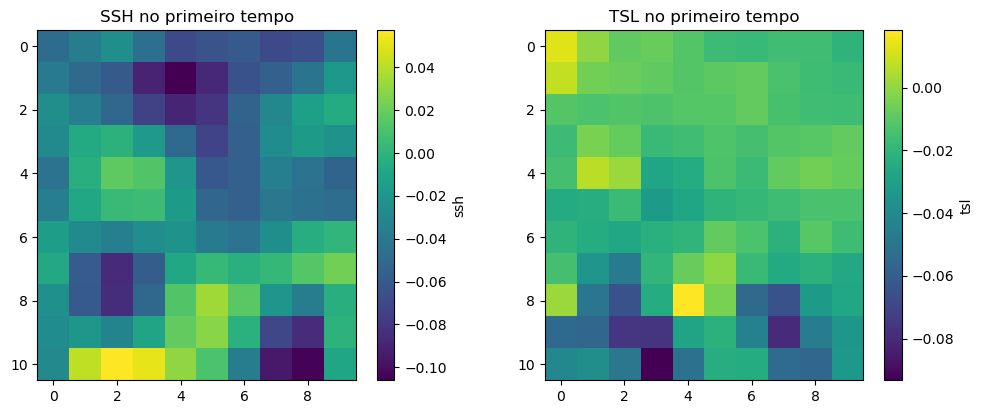
\includegraphics[width=0.9\linewidth]{lista3-1a}
	\caption{Visualização dos dados de ssh e tsl pela função imshow}
	\label{fig:lista3-1a}
\end{figure}

A figura \ref{fig:lista3-1b} apresenta a autocorreção das anomalias de ssh e tsl utilizando uma adaptação da função \textcolor{red}{time\_scale.m} para Python:

\begin{figure}[H]
	\centering
	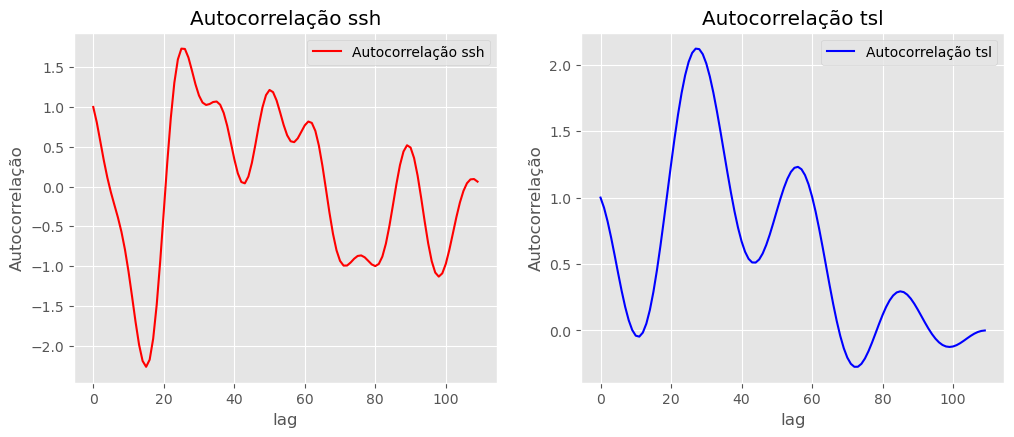
\includegraphics[width=0.9\linewidth]{lista3-1b}
	\caption{Autocorreção das anomalias de ssh e tsl}
	\label{fig:lista3-1b}
\end{figure}
A tabela \ref{tsarr} apresenta as integrais de escala de tempo e os grais de liberdade de cada série

\begin{table}[H]
	\centering
	\begin{tabular}{l|c|c|}
		\cline{2-3}
		& \multicolumn{1}{l|}{Integral de escala de tempo} & \multicolumn{1}{l|}{Grau de Liberdade} \\ \hline
		\multicolumn{1}{|l|}{SSH} & 2.28                                             & 3.5                                    \\ \hline
		\multicolumn{1}{|l|}{TSL} & 4.47                                             & 1.8                                    \\ \hline
	\end{tabular}
	\caption{Integral de escala e graus de liberdade para as séries temporais}
	\label{tsarr}
\end{table}

	Utilizando o código para o cálculo da correlação cruzada em todos os pontos da grade:
	\begin{python}
cor = np.zeros_like(ssh[:,:,0])
for i in range (ssh.shape[0]):
	for j in range (ssh.shape[1]):
		cor[i,j],_ = scipy.stats.pearsonr(ssh[i,j,:],tsl[i,j,:])
	\end{python}
	É possível plotar a figura \ref{fig:lista3-3c}
	
\begin{figure}[H]
	\centering
	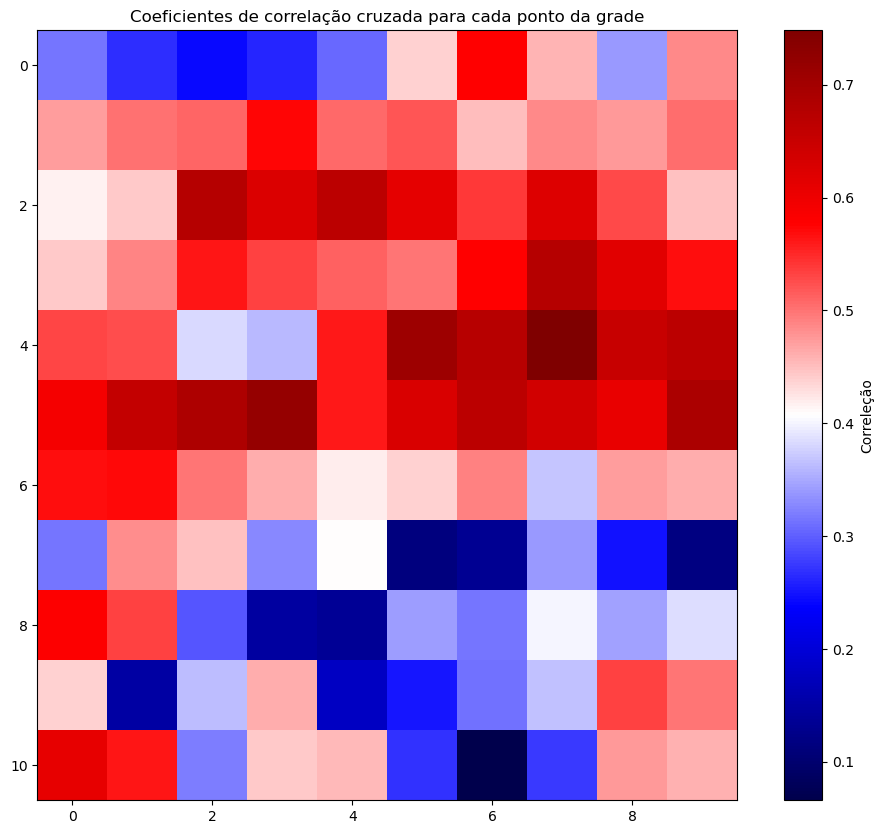
\includegraphics[width=1\linewidth]{lista3-3c}
	\caption{Coeficientes de correlação cruzada de ssh e tsl para cada ponto da grade}
	\label{fig:lista3-3c}
\end{figure}
	
\textbf{Parte II – Periodicidade}
	
Realizando plot dos dados de CO$_2$ para a estação de Mauna Loa, conforme a figura \ref{fig:lista3-4b}, é visível que existe uma tendência nos dados.
\begin{figure}[H]
	\centering
	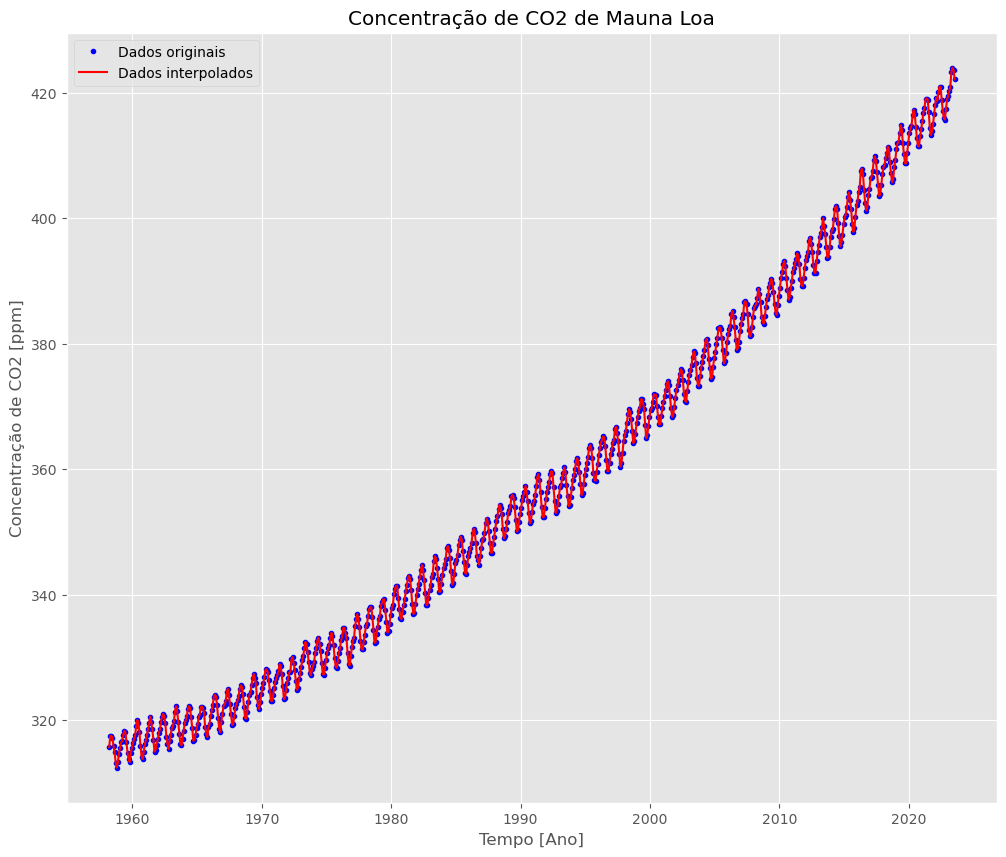
\includegraphics[width=1\linewidth]{lista3-4b}
	\caption{Comparação dos dados originais da Concentração de  CO$_2$ de Mauna Loa com os dados interpolados}
	\label{fig:lista3-4b}
\end{figure}
Utilizando o código para remover a tendência:
\begin{python}
detrend=statsmodels.tsa.tsatools.detrend(co2i, order=3, axis=0)
\end{python}
Se obtém a figura \ref{fig:lista3-4c}
\begin{figure}[H]
	\centering
	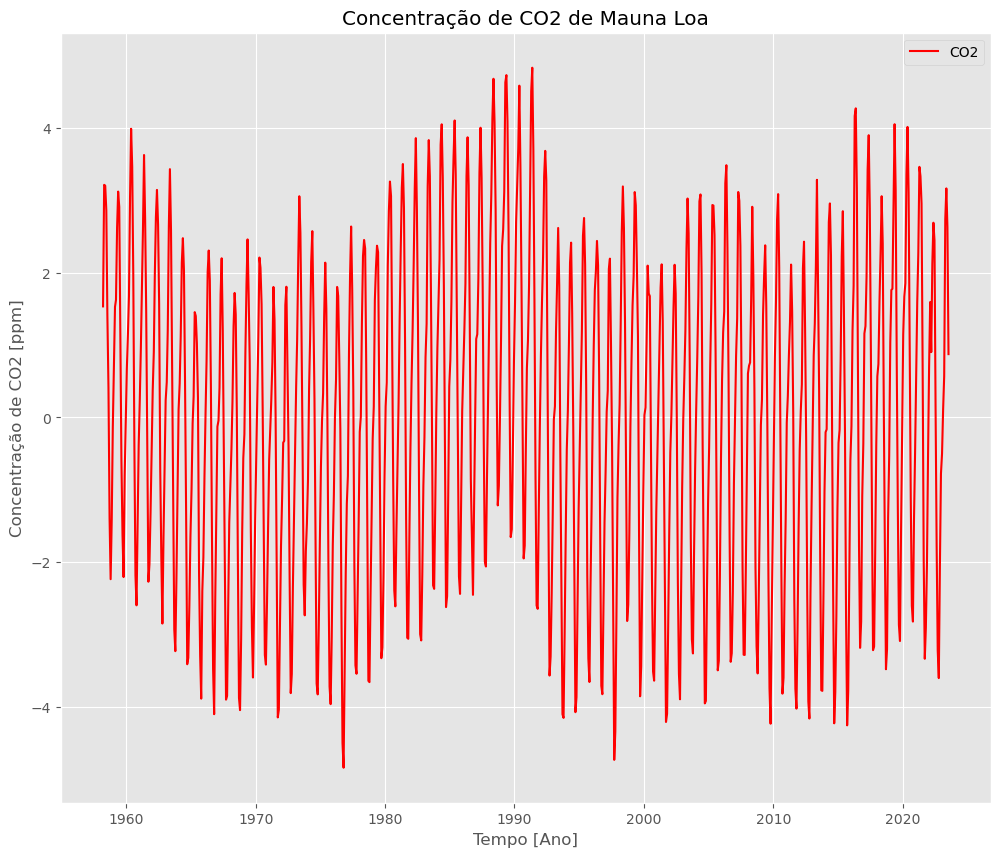
\includegraphics[width=1\linewidth]{lista3-4c}
	\caption{Concentração de  CO$_2$ de Mauna Loa com a tendência linear removida}
	\label{fig:lista3-4c}
\end{figure}
A retirada da tendência linear dos dados parece ter se ajustado bem, com os dados respondendo apenas a uma variação sazonal, porém ainda existe pontos em que a tendência não foi totalmente removida.

A figura \ref{fig:lista3-4d} mostra a curva de ajuste utilizando um polonimo de 3° grau juntamente com os dados da concentração de CO$_2$
\begin{figure}[H]
	\centering
	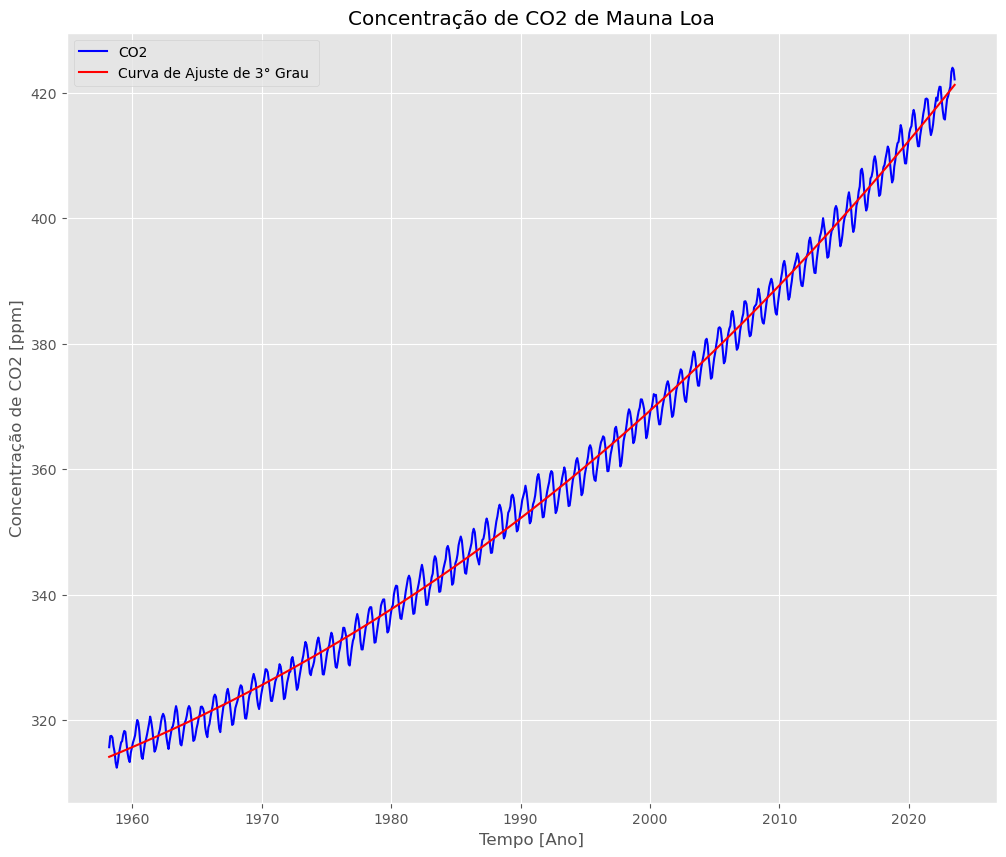
\includegraphics[width=1\linewidth]{lista3-4d}
	\caption{Concentração de  CO$_2$ de Mauna Loa com uma curva de ajuste de 3° grau}
	\label{fig:lista3-4d}
\end{figure}

Repetindo a remoção da tendência dos dados utilizando agora a curva de ajuste, se obtém os resultados da figura \ref{fig:lista3-4e}, onde os dados se mostram com uma melhor remoção da tendência quando comparados com o da figura \ref{fig:lista3-4c}

\begin{figure}[H]
	\centering
	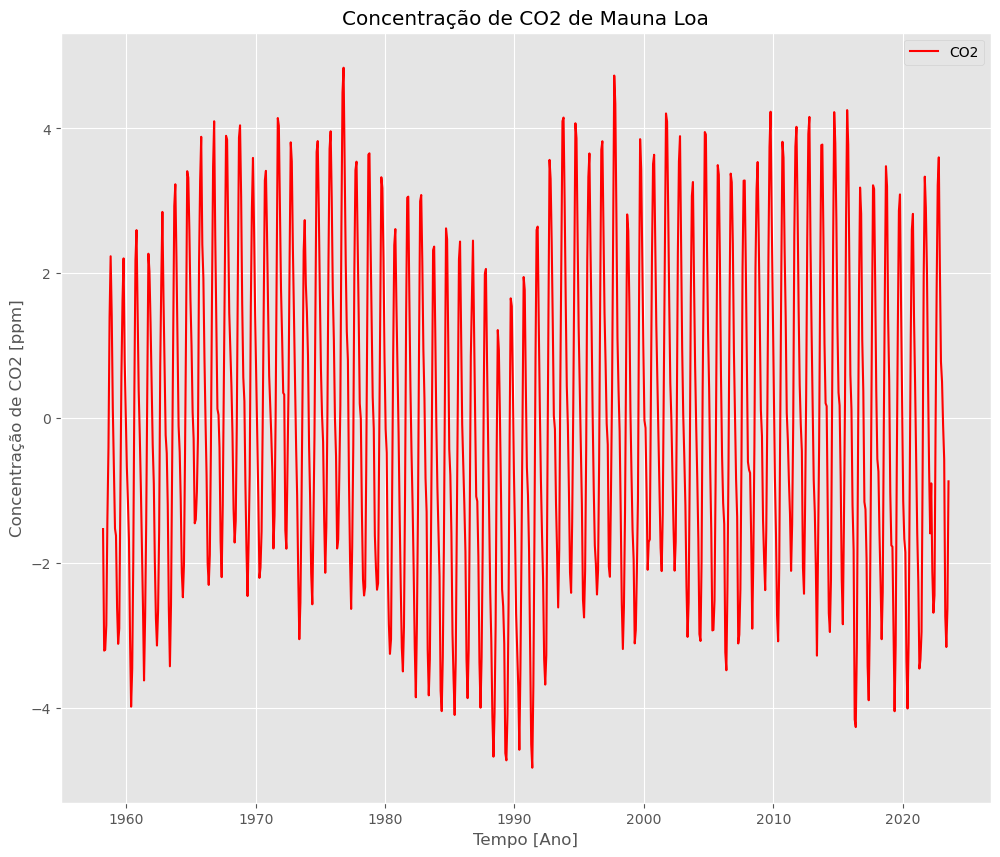
\includegraphics[width=1\linewidth]{lista3-4e}
	\caption{Concentração de  CO$_2$ de Mauna Loa com a tendência removida utilizando uma curva de ajuste}
	\label{fig:lista3-4e}
\end{figure}

Gerando a série com o código:
\begin{python}
dt = 0.5
T = 10
N = 200
t = np.arange(0, N) * dt
y = 2 * np.cos((2 * np.pi / T) * t)
c, lags = np.correlate(y, y, mode='full'), np.arange(-N+1, N)
\end{python}
Essa série vai possuir uma frequência de 2 amostras por segundo, mudando o valor de N, se obtêm:
\begin{figure}[H]
	\centering
	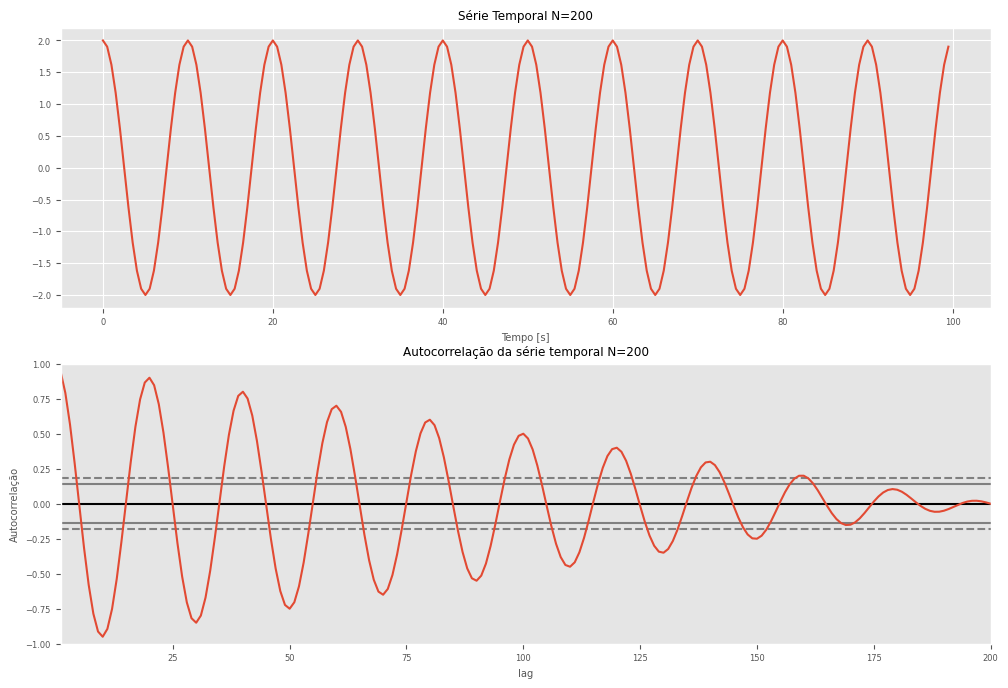
\includegraphics[width=1\linewidth]{lista3-5-200}
	\caption{Série temporal gerada com N=200 e a sua autocorreção }
	\label{fig:lista3-5-200}
\end{figure}

\begin{figure}[H]
	\centering
	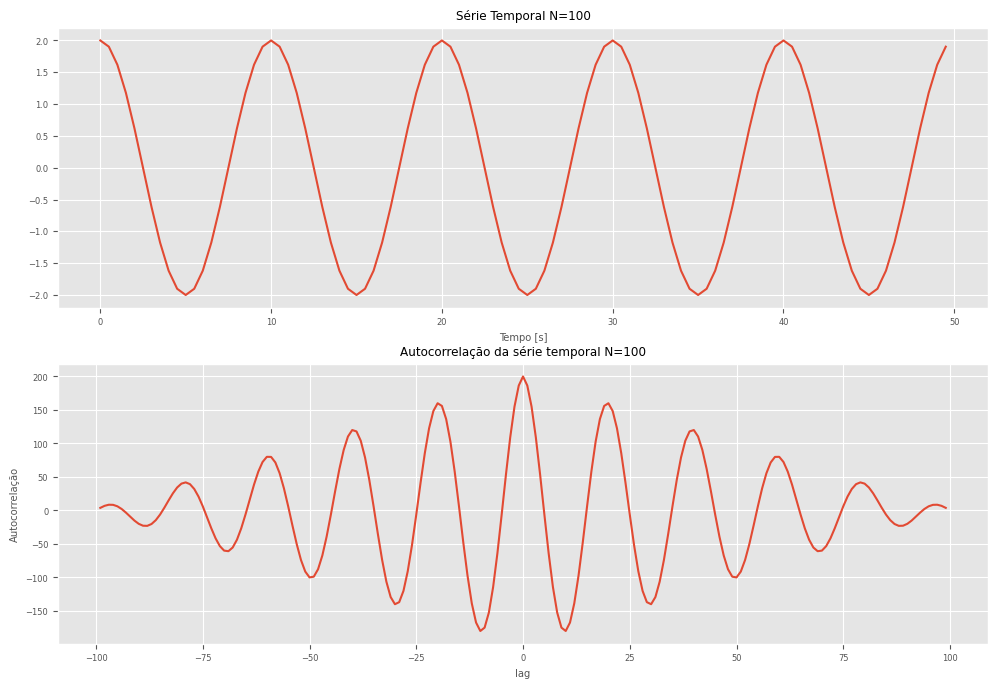
\includegraphics[width=1\linewidth]{lista3-5-100}
	\caption{Série temporal gerada com N=100 e a sua autocorreção }
	\label{fig:lista3-5-100}
\end{figure}

\begin{figure}[H]
	\centering
	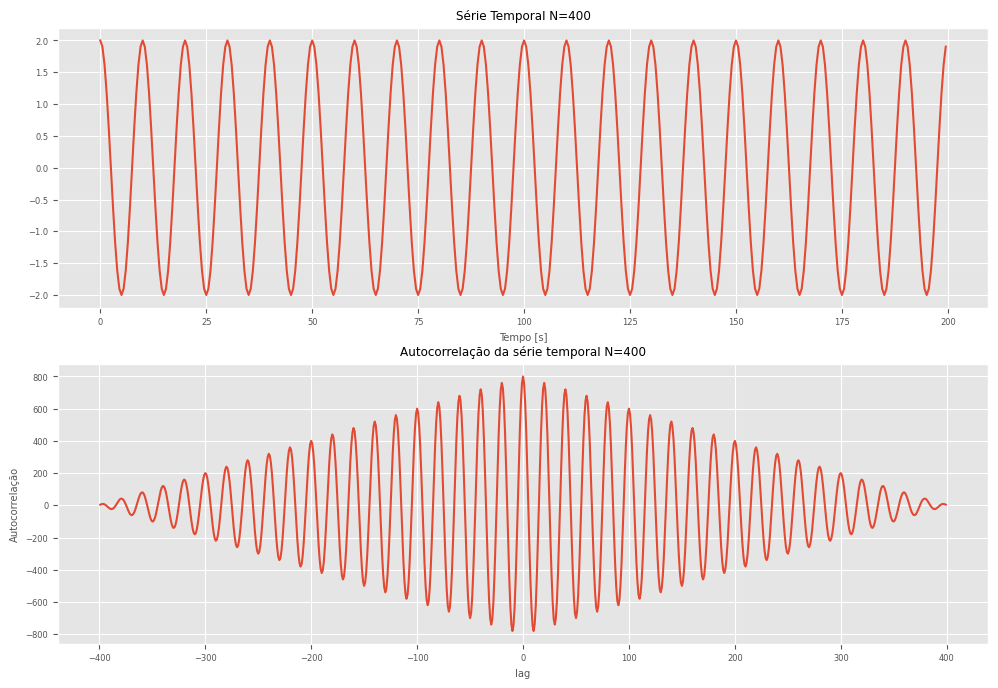
\includegraphics[width=1\linewidth]{lista3-5-400}
	\caption{Série temporal gerada com N=400 e a sua autocorreção }
	\label{fig:lista3-5-400}
\end{figure}

Para a concentração de CO2 de Mauna Loa, a autocorrelação da série original e da série com a tendencia removida é apresentada na figura \ref{fig:lista3-6a}
\begin{figure}[H]
	\centering
	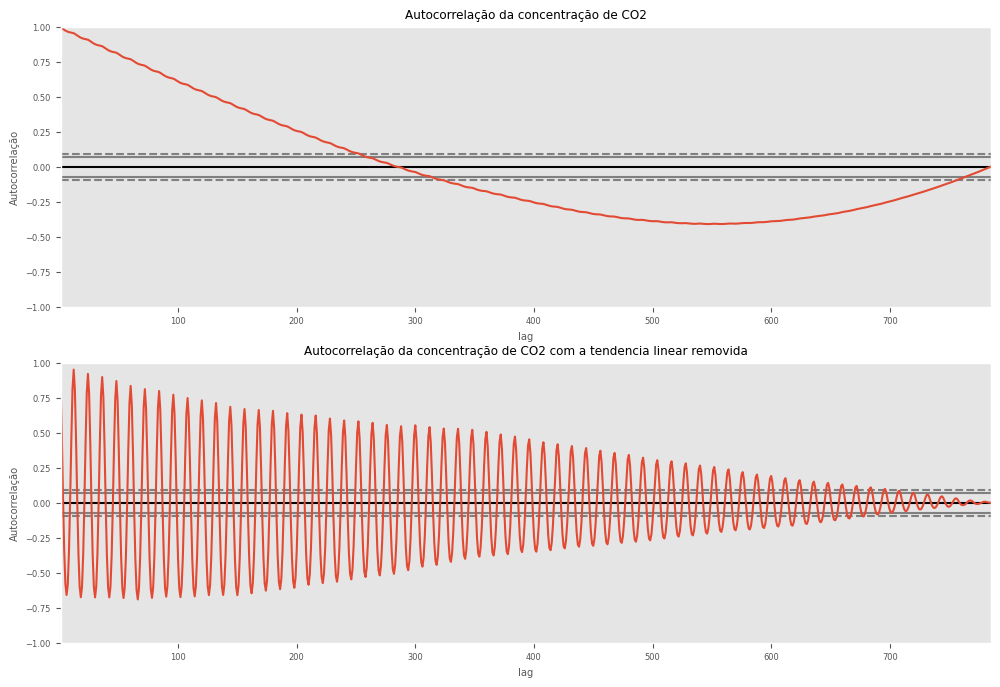
\includegraphics[width=1\linewidth]{lista3-6a}
	\caption{Autocorrelação da concentração de CO2 de Mauna Loa, utilizando os dados originais e os dados com a tendência removida respectivamente}
	\label{fig:lista3-6a}
\end{figure}
Plotando o histograma:
\begin{figure}[H]
	\centering
	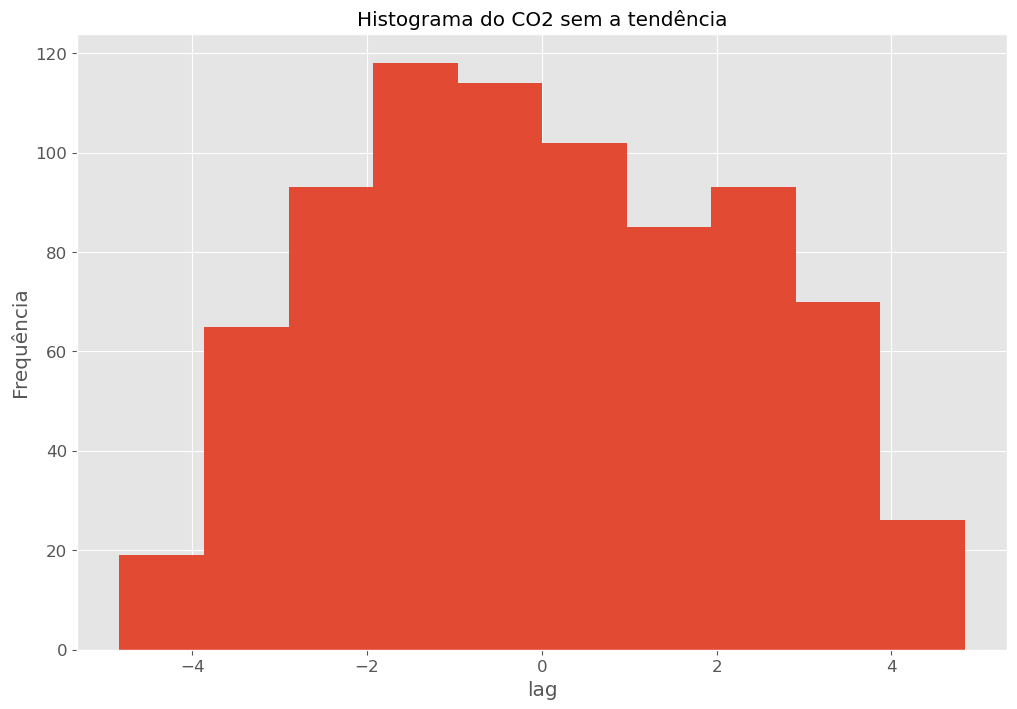
\includegraphics[width=1\linewidth]{lista3-6d}
	\caption{Histograma do CO2 sem a tendência}
	\label{fig:lista3-6d}
\end{figure}
O valor do lillietest é 0.001.

Repetindo para o índice da oscilação sul:


\begin{figure}[H]
	\centering
	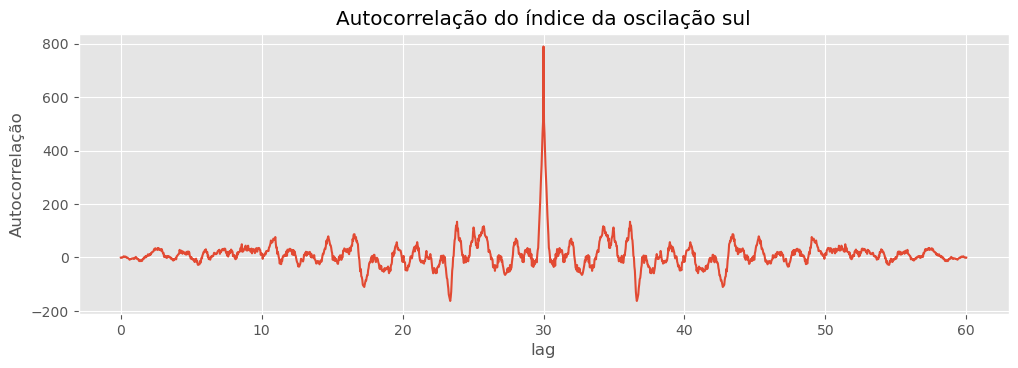
\includegraphics[width=1\linewidth]{lista3-7}
	\caption{Autocorrelação do Índice da oscilação sul}
	\label{fig:lista3-7}
\end{figure}



\end{document}